\section{Structure de séquences répartie à large échelle}

\begin{frame}{Structure de séquences}{Réplication}
  \vspace{-1.5cm}

  La \textbf{réplication optimiste}\footfullcite{saito2005optimistic} améliore
  la \textbf{disponibilité} d'un document et sa \textbf{réactivité} aux
  changements effectués.  \vspace{0.75cm}

  Fonctionnement :
  \begin{enumerate}[(a)]
  \item Une modification produit un résultat;
  \item ce résultat est disséminé aux autres répliques;
  \item ces dernières exécutent -- ou intègrent -- le résultat reçu.
  \end{enumerate}

  \begin{textblock*}{\textwidth}(-0.65cm,0.4cm) 
    
\begin{tikzpicture}[scale=0.95]

  \newcommand\X{30pt};
  \newcommand\Y{30pt};
  
  \draw[->](0pt,   0pt)--(10*\X,   0pt);
  \draw[->](0pt, -1*\Y)--(10*\X, -1*\Y);
  \draw[->](0pt, -2*\Y)--(10*\X, -2*\Y);
  
  \draw[fill=black](0pt, 0pt) node[anchor=east]{éditeur 1 }circle(2pt);
  \draw[fill=black](0pt, -1*\Y) node[anchor=east]{éditeur 2 }circle(2pt);
  \draw[fill=black](0pt, -2*\Y) node[anchor=east]{éditeur 3 }circle(2pt);

  \draw(\X,2pt)--node[anchor=south]{[WERTY]}( \X,   -2pt);
  \draw(\X,2 -1*\Y)--node[anchor=south]{[WERTY]}(\X,-2 -1*\Y);
  \draw(\X,2 -2*\Y)--node[anchor=south]{[WERTY]}(\X,-2 -2*\Y);
  \footnotesize
  \draw(3* \X,2pt)--node[anchor=north]
  {(a) \textsc{insert}(Q, 0) \DARKBLUE{\textbf{produit} $resultat$}}(3 * \X,   -2pt);
%  \draw(3* \X,2 -2*\Y)--node[anchor=north]{\textsc{delete}(\DARKBLUE{\textbf{0}})}(3 * \X,-2 -2*\Y);
  \normalsize

  \draw(3* \X,2pt)--node[anchor=south]{[QWERTY]}(3 * \X,   -2pt);
%  \draw(2* \X,2 -1*\Y)--node[anchor=south]{[ ]}(2* \X,-2 -1*\Y)
%  \draw(3* \X,2 -2*\Y)--node[anchor=south]{[ERTY]}( 3 * \X,-2 -2*\Y);

  \footnotesize
  \draw[->, dashed] (5*\X, 0pt) -- (15+7*\X, -1*\Y);
  \draw[->, dashed] (5*\X, 0pt)
  node[anchor = south west]{(b) \DARKBLUE{\textbf{dissémine}} $resultat$} -- (7*\X, -2*\Y);


  \draw (15+ 7*\X, 2-1*\Y) -- (15+ 7*\X, -2-1*\Y)
  node [anchor=north]{(c)};
  \draw (7*\X, 2-2*\Y) -- (7*\X, -2-2*\Y)
  node [anchor=north]{(c) \DARKBLUE{\textbf{intègre}} $resultat$ };
  \normalsize

%  \draw[->, dashed] (5*\X, -2*\Y) -- (7*\X,  0*\Y)
%  node[anchor=south]{\textsc{delete}(\DARKBLUE{\textbf{0}})};
%  \normalsize
%  \draw[->, dashed] (5*\X, -2*\Y) -- (7*\X, -1*\Y);

  \draw(9*\X, 2 -0*\Y)--node[anchor=south]{[QWERTY]}(9*\X,-2 -0*\Y);
  \draw(9*\X, 2 -1*\Y)--node[anchor=south]{[QWERTY]}(9*\X,-2 -1*\Y);
  \draw(9*\X, 2 -2*\Y)--node[anchor=south]{[QWERTY]}(9*\X,-2 -2*\Y);


%%  \draw(9*\X, 2 -0*\Y)--node[anchor=south]{[QWERTY]}(9*\X,-2 -0*\Y);
%%  \draw(9*\X, 2 -1*\Y)--node[anchor=south]{[QWERTY]}(9*\X,-2 -1*\Y);
%%  \draw(9*\X, 2 -2*\Y)--node[anchor=south]{[QWERTY]}(9*\X,-2 -2*\Y);


%%  \draw[fill=white, very thick]
%%  (0*\X, 0*\Y) node{$p_1$} +(-5pt,-5pt) rectangle +(5pt,5pt);
%%  \draw[->](-5+\X, 5+2*\Y)to[out=120,in=30](0pt,5+2*\Y); %% 6 -> 7
\end{tikzpicture}
  \end{textblock*}
  
  \vspace{1cm}

\end{frame}


\begin{frame}{Structure de séquences}{Cohérence des répliques}
  
  \vspace{-1.5cm}

  D'après Sun et al.\footfullcite{sun1998achieving}, l'édition collaborative
  temps réel nécessite un système préservant les trois propriétés :

  \begin{itemize}
  \item Convergence;
  \item Causalité;
  \item Intention.  
  \end{itemize}

  \begin{textblock*}{\textwidth}(-0.65cm,0.4cm) 
    
\begin{tikzpicture}[scale=0.95]

  \newcommand\X{30pt};
  \newcommand\Y{30pt};
  
  \draw[->](0pt,   0pt)--(10*\X,   0pt);
  \draw[->](0pt, -1*\Y)--(10*\X, -1*\Y);
  \draw[->](0pt, -2*\Y)--(10*\X, -2*\Y);
  
  \draw[fill=black](0pt, 0pt) node[anchor=east]{réplique 1 }circle(2pt);
  \draw[fill=black](0pt, -1*\Y) node[anchor=east]{réplique 2 }circle(2pt);
  \draw[fill=black](0pt, -2*\Y) node[anchor=east]{réplique 3 }circle(2pt);

  \draw(\X,2pt)--node[anchor=south]{[WERTY]}( \X,   -2pt);
  \draw(\X,2 -1*\Y)--node[anchor=south]{[WERTY]}(\X,-2 -1*\Y);
  \draw(\X,2 -2*\Y)--node[anchor=south]{[WERTY]}(\X,-2 -2*\Y);
  \footnotesize
  \draw(3* \X,2pt)--node[anchor=north]
  {\textsc{insert}(Q, 0)}(3 * \X,   -2pt);
%  \draw(3* \X,2 -2*\Y)--node[anchor=north]{\textsc{delete}(\DARKBLUE{\textbf{0}})}(3 * \X,-2 -2*\Y);
  \normalsize

  \draw(3* \X,2pt)--node[anchor=south]{[QWERTY]}(3 * \X,   -2pt);
%  \draw(2* \X,2 -1*\Y)--node[anchor=south]{[ ]}(2* \X,-2 -1*\Y)
%  \draw(3* \X,2 -2*\Y)--node[anchor=south]{[ERTY]}( 3 * \X,-2 -2*\Y);

  \footnotesize
  \draw[->, dashed] (4*\X, 0pt) -- (4.5*\X, -1*\Y);
  \draw[->, dashed] (4*\X, 0pt) to[out=25,in=155] (7.5*\X, 0pt)
  to[out=-40,in=95] (8.2*\X, -2*\Y);
  
  \draw(5.5*\X, 2-1*\Y)node[anchor=south]{\normalsize[WERTY]}--(5.5*\X, -2-1*\Y)
  node[anchor=north]{\footnotesize\textsc{delete}(0)};

  \draw[->, dashed] (6.5*\X, -1*\Y) -- (7*\X, -0*\Y);
  \draw[->, dashed] (6.5*\X, -1*\Y) -- (7*\X, -2*\Y);

  \draw[->, dashed, color=darkblue] (7*\X, -2*\Y) to[out=-45,in=-135]
  node[anchor=north]{\DARKBLUE{\textbf{attend}}} (8.5*\X, -2*\Y);

  \normalsize

%  \draw[->, dashed] (5*\X, -2*\Y) -- (7*\X,  0*\Y)
%  node[anchor=south]{\textsc{delete}(\DARKBLUE{\textbf{0}})};
%  \normalsize
%  \draw[->, dashed] (5*\X, -2*\Y) -- (7*\X, -1*\Y);

  \draw(9*\X, 2 -0*\Y)--node[anchor=south]{[WERTY]}(9*\X,-2 -0*\Y);
  \draw(9*\X, 2 -1*\Y)--node[anchor=south]{[WERTY]}(9*\X,-2 -1*\Y);
  \draw(9*\X, 2 -2*\Y)--node[anchor=south]{[WERTY]}(9*\X,-2 -2*\Y);


%%  \draw(9*\X, 2 -0*\Y)--node[anchor=south]{[QWERTY]}(9*\X,-2 -0*\Y);
%%  \draw(9*\X, 2 -1*\Y)--node[anchor=south]{[QWERTY]}(9*\X,-2 -1*\Y);
%%  \draw(9*\X, 2 -2*\Y)--node[anchor=south]{[QWERTY]}(9*\X,-2 -2*\Y);


%%  \draw[fill=white, very thick]
%%  (0*\X, 0*\Y) node{$p_1$} +(-5pt,-5pt) rectangle +(5pt,5pt);
%%  \draw[->](-5+\X, 5+2*\Y)to[out=120,in=30](0pt,5+2*\Y); %% 6 -> 7
\end{tikzpicture}
  \end{textblock*}

\end{frame}


\begin{frame}{Structure de séquences}{Intention}
  
  L'effet observé sur le document lors de la génération d'une opération doit
  être également observé lors de son intégration malgré l'interférence
  d'opérations \textbf{concurrentes}.

  \vspace{0.5cm}

  \begin{itemize}
  \item Difficile à formaliser dans le cas général;
  \item L'opération doit respecter le plus possible sa spécification
    séquentielle \footfullcite{bieniusa2012brief}.
  \end{itemize}

  \vspace{0.5cm}
  
  Pour la séquence :
  \begin{itemize}
  \item \og insérer l'élément $e$ à la position $i$ dans la séquence \fg
  \item \og supprimer l'élément à la position $i$ dans la séquence \fg
  \end{itemize}

  \vspace{0.5cm}

  \begin{itemize}
    \only<1-1>{\item [$\rightarrow$]L'intention semble être liée aux
      positions.}
    \only<2->{\item [$\rightarrow$]\sout{L'intention semble être
        liée aux \textbf{positions}.}}
    \uncover<2->{\item [$\rightarrow$] Une séquence
    se définit par un \textbf{ordre dense} sur ses éléments : les éléments 
    sont ordonnés
    et il est toujours possible d'insérer un élément entre deux autres éléments.}
  \end{itemize}

  \vspace{0.2cm}
  
\end{frame}

\begin{frame}{Structure de séquences}{Spécification}
  \begin{definition}[Spécification séquentielle d'une séquence]
  Soit une série d'opérations $H$ produisant la séquence
  $s(H) = \{p_1,\, p_2 \ldots p_k\}$ avec $p_{1..k} \in \mathcal{P}$ où
  $\mathcal{P}$ est un ensemble muni d'un ordre
  dense $(\mathcal{P},\,<_\mathcal{P})$ tel que : \\
  $\forall p\in\mathcal{P},\, p_\vdash <_\mathcal{P} p <_\mathcal{P} p_\dashv $
  \hfill et \ \
  $p_\vdash <_\mathcal{P} p_1 <_\mathcal{P} p_2 <_\mathcal{P} \ldots
  <_\mathcal{P} p_k <_\mathcal{P} p_\dashv$.
  
  \vspace{0.25cm}

  \noindent L'insertion d'un élément $e$ en position $i$ dans la séquence $s(H)$
  est définie de la façon suivante :
  \begin{equation}
    \small
    s(H \cup INSERT(i,\, e)) \rightarrow s(H) \cup 
    \begin{cases}
      \{p,\, p_\vdash <_\mathcal{P} p <_\mathcal{P} p_\dashv \} & i = 0 \wedge |s(H)| = 0\\
      \{p,\, p_\vdash <_\mathcal{P} p <_\mathcal{P} p_1 \} & i = 0 \wedge |s(H)|>0\\
      \{p,\, p_k <_\mathcal{P} p <_\mathcal{P} p_\dashv \} & i = k\\
      \{p,\, p_i <_\mathcal{P} p <_\mathcal{P} p_{i+1} \} & sinon
    \end{cases}
  \end{equation}

  \noindent La suppression de l'élément en position $i$ dans la séquence $s(H)$
  est définie de la façon suivante :
  \begin{equation}
    \small
    s(H \cup DELETE(i)) \rightarrow s(H) \setminus \{ p_i \}
  \end{equation}
\end{definition}
\end{frame}


\begin{frame}{Structure de séquences}{Complexités}

Créer un ordre dense a un coût dont la progression peut être estimée par : 

\vspace{0.5cm}

\begin{itemize}
  \only<1-1>{\item Complexité en \textbf{communication};}
  \only<2->{\item  \textbf{Complexité en communication};}
\item Complexité \textbf{spatiale} de la réplique;
\item Complexité \textbf{temporelle} d'une opération \textbf{générée} localement;
  \only<1-1>{\item Complexité \textbf{temporelle} de l'\textbf{intégration} d'une opération reçue.}
  \only<2->{\item \textbf{Complexité temporelle de l'intégration d'une opération reçue.}}
\end{itemize}

%% (TODO) maybe explain the reasons of this emphasis
\end{frame}


% \begin{frame}{Structure de séquences}{État de l'art : transformées opérationnelles}

%   \vspace{-1.5cm}

%   Ces approches \REF{} ont une signature identique à celle communément employée
%   pour les séquences : 
%   \begin{itemize}
%   \item \textsc{insert}($element,\,position$)
%   \item \textsc{delete}($position$)
%   \end{itemize}

%   \vspace{0.5cm}

%   Lors de la réception d'une opération, ses arguments sont ajustés afin qu'ils
%   s'appliquent à l'état courant de la réplique malgré les opérations effectuées
%   et intégrées en concurrence. 


%   \begin{textblock*}{\textwidth}(-0.65cm,0.4cm) 
%     
\begin{tikzpicture}[scale=0.95]

  \newcommand\X{30pt};
  \newcommand\Y{30pt};
  
  \draw[->](0pt,   0pt)--(10*\X,   0pt);
  \draw[->](0pt, -1*\Y)--(10*\X, -1*\Y);
  \draw[->](0pt, -2*\Y)--(10*\X, -2*\Y);
  
  \draw[fill=black](0pt, 0pt) node[anchor=east]{réplique 1 }circle(2pt);
  \draw[fill=black](0pt, -1*\Y) node[anchor=east]{réplique 2 }circle(2pt);
  \draw[fill=black](0pt, -2*\Y) node[anchor=east]{réplique 3 }circle(2pt);

  \draw(\X,2pt)--node[anchor=south]{[WERTY]}( \X,   -2pt);
  \draw(\X,2 -1*\Y)--node[anchor=south]{[WERTY]}(\X,-2 -1*\Y);
  \draw(\X,2 -2*\Y)--node[anchor=south]{[WERTY]}(\X,-2 -2*\Y);
  \footnotesize
  \draw(3* \X,2pt)--node[anchor=north]{\textsc{insert}(Q, 0)}(3 * \X,   -2pt);
  \draw(3* \X,2 -2*\Y)--node[anchor=north]{\textsc{delete}(\DARKBLUE{\textbf{0}})}(3 * \X,-2 -2*\Y);
  \normalsize

  \draw(3* \X,2pt)--node[anchor=south]{[QWERTY]}(3 * \X,   -2pt);
%  \draw(2* \X,2 -1*\Y)--node[anchor=south]{[ ]}(2* \X,-2 -1*\Y)
  \draw(3* \X,2 -2*\Y)--node[anchor=south]{[ERTY]}( 3 * \X,-2 -2*\Y);

  \draw[->, dashed] (5*\X, 0pt) -- (7*\X, -1*\Y);
  \draw[->, dashed] (5*\X, 0pt) -- (7*\X, -2*\Y);

  \footnotesize
  \draw[->, dashed] (5*\X, -2*\Y) -- (7*\X,  0*\Y)
  node[anchor=south]{\textsc{delete}(\DARKBLUE{\textbf{1}})};
  \normalsize
  \draw[->, dashed] (5*\X, -2*\Y) -- (7*\X, -1*\Y);

  \draw(9*\X, 2 -0*\Y)--node[anchor=south]{[QERTY]}(9*\X,-2 -0*\Y);
  \draw(9*\X, 2 -1*\Y)--node[anchor=south]{[QERTY]}(9*\X,-2 -1*\Y);
  \draw(9*\X, 2 -2*\Y)--node[anchor=south]{[QERTY]}(9*\X,-2 -2*\Y);


%%  \draw(9*\X, 2 -0*\Y)--node[anchor=south]{[QWERTY]}(9*\X,-2 -0*\Y);
%%  \draw(9*\X, 2 -1*\Y)--node[anchor=south]{[QWERTY]}(9*\X,-2 -1*\Y);
%%  \draw(9*\X, 2 -2*\Y)--node[anchor=south]{[QWERTY]}(9*\X,-2 -2*\Y);


%%  \draw[fill=white, very thick]
%%  (0*\X, 0*\Y) node{$p_1$} +(-5pt,-5pt) rectangle +(5pt,5pt);
%%  \draw[->](-5+\X, 5+2*\Y)to[out=120,in=30](0pt,5+2*\Y); %% 6 -> 7
\end{tikzpicture}
%   \end{textblock*}
% \end{frame}


\begin{frame}{Structure de séquences}{Le prix de la causalité}
  
  Ordonner les opérations selon l'ordre causal est extrêmement coûteux : au
  minimum $\mathcal{O}(W)$ en communication où $W$ est le nombre de participants
  ayant jamais écrit dans le document \footfullcite{charronbost1991concerning}.
  \begin{itemize}
  \item[$\rightarrow$] Relaxer l'ordre est nécessaire pour le passage à l'échelle
  \end{itemize}
  
  \vspace{0.5cm}
  
  \large
  \begin{itemize}
  \item [$\rightarrow$] L'utilisation de structures de données répliquées sans
    conflits \footfullcite{shapiro2011conflict} permet cela.
    \begin{itemize}
    \item [$\rightarrow$] Ces approches se basent sur la génération
      d'identifiants uniques et immuables. Nous nous intéresserons
      particulièrement à celles dont les identifiants sont des listes de taille
      variable.
    \end{itemize}
  \end{itemize}

\end{frame}

\begin{frame}{Structure de séquences}{Structures sans conflits}
  
  La signature change : 
  \begin{itemize}
  \item \textsc{insert}($element,\, position$) $\rightarrow$
    \textsc{insert}($id_{position-1},\, element,\, id_{position}$)
  \item \textsc{delete}($position$) $\rightarrow$ \textsc{delete}($id_{position}$)
  \end{itemize}

  \vspace{0.5cm}
  

  \begin{algorithm}[H]
    
\footnotesize
\algrenewcommand{\algorithmiccomment}[1]{\hskip2em$\rhd$ #1}

\newcommand{\comment}[1]{$\rhd$ #1}


\algblockdefx[initially]{initially}{endInitially}
  [0] {\textbf{INITIALLY:}} 

\algblockdefx[local]{local}{endLocal}
  [0] {\textbf{LOCAL UPDATE:}}

\algsetblockdefx[received]{received}{endReceived}
  {65535}{}
  [0] {\textbf{RECEIVED UPDATE:}}

\algblockdefx[onInsert]{onLocal}{endOnLocal}
  [0] {\textbf{on} insert ($previous \in \mathcal{I},\,\alpha \in \mathcal{A},\,
   next\in\mathcal{I}$):}
  [0] {\textbf{on} delete ($i \in \mathcal{I}$):} 

\algsetblockdefx[onRemote]{onRemote}{endOnRemote}
  {65535}{}
  [0] {\textbf{on} insert ($i\in\mathcal{I}$):
    \hfill\comment{\DARKBLUE{\textbf{une fois}} par identifiant}}
  [0] {\textbf{on} delete ($i\in\mathcal{I}$):
    \hfill\comment{\DARKBLUE{\textbf{après}} l'exécution de \textsc{insert}($i$)}} 

\newcommand{\LINEFOR}[2]{%
  \algorithmicfor\ {#1}\ \algorithmicdo\ {#2} %
  }

\newcommand{\LINEIFTHEN}[2]{%
  \algorithmicif\ {#1}\ \algorithmicthen\ {#2} %
  }

\newcommand{\INDSTATE}[1][1]{\State\hspace{\algorithmicindent}}

\begin{algorithmic}[1]
  \Statex
  \initially
    \State $T \leftarrow \varnothing$;
    \hfill \comment{CRDT conçue pour les séquences}
  \endInitially
  
  \local
    \onLocal
    \State \textbf{let}
    $\langle p,\, q \rangle \leftarrow $\textsc{convert2Path}$(previous,\, next)$;
    \State \textbf{let}
    $\DARKBLUE{newPath \leftarrow} $\DARKBLUE{\textbf{\textsc{allocPath}}}\DARKBLUE{$(p,\,q)$}; \label{line:allocpath}
    \State \textbf{let} 
    $newDis \leftarrow $\textsc{allocDis}$(p,\, newPath,\, q)$; \label{line:allocdes}
    \State \textsc{broadcast}$(\text{'insert'},\,
    \langle newPath,\, \alpha,\, newDis \rangle)$;
    \endOnLocal
    \INDSTATE \textsc{broadcast}$(\text{'delete'},\,i)$;
  \endLocal
  
  \received
    \onRemote
    \State $T \leftarrow T \cup i$;
    \endOnRemote
    \INDSTATE $T \leftarrow T\, \backslash\, i$; 
  
\end{algorithmic}

  \end{algorithm}

\end{frame}


\begin{frame}{Structure de séquences}{Problèmes d'allocation}

  La fonction d'allocation ne connait ni le \textbf{nombre} de caractères, ni
  leur \textbf{position} dans la séquence finale.
  
  \vspace{0.5cm}

  \begin{center}
    \begin{tikzpicture}

  \draw(-4,1)node{0};

  \draw[hide on=1-5, bold on=6](-3,1)node{0.0.0.1};
  \draw[hide on=1-4, bold on=5](-2,1)node{0.0.1};
  \draw[hide on=1-3, bold on=4](-1,1)node{0.1};
  \draw[bold on=1](0,1)node{1};
  \draw[hide on=1, bold on=2](1,1)node{2};
  \draw[hide on=1-2,bold on=3](2,1)node{3};
%  \draw[hide on=1-2,bold on=3](3,1)node{8};
%  \draw[hide on=1-3,bold on=4](4,1)node{8.1};

  \draw(5,1)node{9};

  \draw[hide on=1-5, bold on=6](-3,0)node{Q};
  \draw[hide on=1-4, bold on=5](-2,0)node{W};
  \draw[hide on=1-3, bold on=4](-1,0)node{E};
  \draw[bold on=1](0,0)node{R};
  \draw[hide on=1, bold on=2](1,0)node{T};
  \draw[hide on=1-2, bold on=3](2,0)node{Y};
%  \draw[hide on=1-2, bold on=3](3,0)node{E};
%  \draw[hide on=1-2, bold on=3](4,0)node{S};


\end{tikzpicture}
  \end{center}

\end{frame}


\begin{frame}{Structure de séquences}{Arbre}
  
  \begin{center}
    \begin{tikzpicture}[scale=1.2]

\newcommand\Y{-30}
\newcommand\ADDY{-8}


  %% node to node
  \small
  \draw[thick] (0pt,0pt) -- node[anchor=south east]{\DARKBLUE{0}} (-40pt,\Y pt);
  \draw[thick] (0pt,0pt) -- node[anchor=east]{3} (30pt, \Y pt); %% Y
  \draw[thick] (0pt, 0 pt) -- node[anchor=east]{2} (15pt, 1 * \Y pt); %% T
  \draw[thick] (-40pt, \Y pt) -- node[anchor=east]{\DARKBLUE{0}} (-40pt, 2 * \Y pt); %% 0
  \draw[thick] (0pt, 0 pt) -- node[anchor=east]{1} (0pt, 1 * \Y pt); %% R
  \draw[thick] (-40pt, 2*\Y pt)-- node[anchor=east]{\DARKBLUE{0}}(-40pt, 3 * \Y pt); %% 0
  \draw[thick] (-40pt, 1*\Y pt) -- node[anchor=north]{1}(-15pt, 2*\Y pt); %% E
  % \draw[thick] (-40pt, 3*\Y pt) -- node[anchor=east]{\DARKBLUE{0}}(-40pt,4 * \Y pt); %% 0
  \draw[thick] (-40pt, 2*\Y pt) -- node[anchor=north]{1}(-25pt, 3* \Y pt); %% W
  % \draw[thick] (-40pt, 4*\Y pt) -- node[anchor=east]{\DARKBLUE{0}}(-40pt,5 * \Y pt); %% 0
  \draw[thick] (-40pt, 3*\Y pt) -- node[anchor=east]{\DARKBLUE{1}}(-35pt, 4*\Y pt); %% Q

  \draw[dashed, thick] (0pt,0pt) -- node[anchor=south west]{9} (40pt,\Y pt);

  %% node to element
  \draw[->] ( 30pt, \Y pt) -- ( 30pt, \ADDY + \Y pt); %% Y
  \draw[->] ( 15pt, 1* \Y pt) -- ( 15pt, \ADDY +  1*\Y pt); %% T
  \draw[->] (  0pt, 1 *\Y pt) -- (  0pt, \ADDY +  1 *\Y pt); %% R
  \draw[->] (-15pt, 2 *\Y pt) -- ( -15pt, \ADDY + 2 *\Y pt); %% E
  \draw[->] (-25pt, 3 *\Y pt) -- ( -25pt, \ADDY + 3 *\Y pt); %% W
  \draw[->] (-35pt, 4 *\Y pt) -- ( -35pt, \ADDY + 4 *\Y pt); %% Q

  %% element to desambiguator
  % \draw[->,densely dashdotted]
  % ( 30pt, \ADDY + \Y pt) -- ( 30pt,2.75*\ADDY+\Y pt); %% Y
  % \draw[->,densely dashdotted]
  % ( 15pt, \ADDY + 2* \Y pt) -- ( 15pt,2.75*\ADDY+ 2* \Y pt); %% T
  % \draw[->,densely dashdotted]
  % ( 0pt, \ADDY + 3* \Y pt) -- (  0pt,2.75*\ADDY+ 3* \Y pt); %% R
  % \draw[->,densely dashdotted]
  % ( -15pt, \ADDY + 4 *\Y pt) -- ( -15pt,2.75*\ADDY+ 4* \Y pt); %% E
  % \draw[->,densely dashdotted]
  % ( -25pt, \ADDY + 5 *\Y pt) -- ( -25pt,2.75*\ADDY+ 5*\Y pt); %% W
  % \draw[->,densely dashdotted]
  % ( -35pt, \ADDY + 6* \Y pt) -- ( -35pt,2.75*\ADDY+ 6*\Y pt); %% Q

  %% node
 \draw[fill=black] (0pt,0pt) circle (1pt); %% rooot
  \draw[fill=white] ( 30pt, \Y pt) circle (1pt); %% Y
  \draw[fill=white] (-40pt, \Y pt) circle (1pt); %% 0
  \draw[fill=white] ( 15 pt, 1 * \Y pt) circle (1pt); %% T
  \draw[fill=white] (-40pt, 2 * \Y pt) circle (1pt); %% 0
  \draw[fill=white] (  0 pt, 1 * \Y pt) circle (1pt); %% R
  \draw[fill=white] (-40pt, 3 * \Y pt) circle (1pt); %% 0
  \draw[fill=white] (-15 pt, 2 * \Y pt) circle (1pt); %% E
%  \draw[fill=white] (-40pt, 4 * \Y pt) circle (1pt); %% 0
  \draw[fill=white] (-25 pt, 3 * \Y pt) circle (1pt); %% W
%  \draw[fill=white] (-40pt, 5 * \Y pt) circle (1pt); %% 0
  \draw[fill=white] (-35 pt, 4 * \Y pt) circle (1pt); %% Q

  \draw[fill=black] ( 40pt, \Y pt) circle (1pt);


  %% elements
  \draw[fill=white] ( 30pt, -4 + \ADDY + \Y pt)
  node{\textbf{Y}} +(-4pt,-4pt) rectangle +(4pt,4pt) ; %% Y
  \draw[fill=white] ( 15pt, -4 + \ADDY +  1 *\Y pt)
  node{\textbf{T}} +(-4pt,-4pt) rectangle +(4pt,4pt) ; %% T
  \draw[fill=white] (  0pt, -4 + \ADDY +  1* \Y pt)
  node{\textbf{R}} +(-4pt,-4pt) rectangle +(4pt,4pt) ; %% R
  \draw[fill=white] (-15pt, -4 + \ADDY + 2 *\Y pt)
  node{\textbf{E}} +(-4pt,-4pt) rectangle +(4pt,4pt) ; %% E
  \draw[fill=white] (-25pt, -4 + \ADDY + 3 * \Y pt)
  node{\textbf{W}} +(-4pt,-4pt) rectangle +(4pt,4pt) ; %% W
  \draw[fill=white] (-35pt, -4 + \ADDY + 4 *\Y pt)
  node{\textbf{Q}} +(-4pt,-4pt) rectangle +(4pt,4pt) ; %% Q

  %% desambiguator
  % \draw[fill=gray!20]( 30pt, -2.5 + 2.75 * \ADDY + \Y pt)
  % +(-2.5pt,-2.5pt) rectangle +(2.5pt,2.5pt);
  % \draw[fill=gray!20]( 15pt, -2.5 + 2.75 * \ADDY +2 *\Y pt)
  % +(-2.5pt,-2.5pt) rectangle +(2.5pt,2.5pt);
  % \draw[fill=gray!20](  0pt, -2.5 + 2.75 * \ADDY + 3*\Y pt)
  % +(-2.5pt,-2.5pt) rectangle +(2.5pt,2.5pt);
  % \draw[fill=gray!20](-15pt, -2.5 + 2.75 * \ADDY +4*\Y pt )
  % +(-2.5pt,-2.5pt) rectangle +(2.5pt,2.5pt);
  % \draw[fill=gray!20](-25pt, -2.5 + 2.75 * \ADDY + 5*\Y pt)
  % +(-2.5pt,-2.5pt) rectangle +(2.5pt,2.5pt);
  % \draw[fill=gray!20](-35pt, -2.5 + 2.75 * \ADDY +6*\Y pt) 
  % +(-2.5pt,-2.5pt) rectangle +(2.5pt,2.5pt);

  %% insertion order
  \draw[->,dashed, color=darkblue] (0pt, 1.75 * \Y pt) node[anchor=north west, align=left]{\ \ \DARKBLUE{ordre}\\ \DARKBLUE{d'insertion}} --  (45pt, 1.75 * \Y pt);

  \draw[->,dashed, color=darkblue] (0pt, 1.75 * \Y pt) -- (-25pt, 4.75 * \Y pt);

\end{tikzpicture}

  \end{center}
  
  \vspace{0.5cm}
  
  La taille des chemins impacte les performances de l'éditeur et le trafic
  généré par l'éditeur.
  \begin{itemize}
  \item [$\rightarrow$] \textsc{allocPath} doit allouer les plus petits chemins
    possibles.
  \end{itemize}

\end{frame}


\begin{frame}{Structure de séquences}{Définition du problème}

  \begin{problem}
    Soit la séquence d'identifiants $s(I)= id_1.id_2\ldots id_I$, et
    $s(I+1) = s(I) \cup $\textsc{insert}$(p,\, \_,\, n)$ où $p,q \in s(I)$ et
    $p<_\mathcal{I}q$. Soit $|s(I)|$ la taille de la représentation binaire de la
    séquence. La fonction \textsc{insert} doit allouer des identifiants tels que :
    \begin{equation}
      |s(I+1)| - |s(I)| < \mathcal{O}(I)
    \end{equation}
  \end{problem}
  
  \vspace{0.5cm}

  \begin{itemize}
  \item [$\rightarrow$] Sinon, il faut relocaliser les identifiants qui ont été
    générés pour conserver de bonnes performances
    \begin{itemize}
    \item [$\approx$] consensus répartis qui ne passe pas à l'échelle.
    \end{itemize}
  \end{itemize}

\end{frame}


\begin{frame}{Structure de séquences}{\LSEQ}
  
  Fonction d'allocation de chemins :
  \begin{enumerate}
  \item Une structure d'arbre dont l'arité maximale augmente avec la profondeur;
  \item Deux sous-fonctions d'allocation conçues pour gérer des comportements
    d'édition opposés;
  \item Une fonction assignant à chaque profondeur de l'arbre une sous-fonction
    d'allocation parmi celles disponibles.
  \end{enumerate}
  
\end{frame}


\begin{frame}{Structure de séquences}{Arbre exponentiel}

  \begin{center}
    
\begin{tikzpicture}[scale=1.3]

\newcommand\X{20pt}
\newcommand\Y{-20pt}

\newcommand\ADDYA{-10pt}
\newcommand\ADDYB{-30pt}

%\draw (-0.5*\X, 0*\Y); %% spacing

\draw[color=darkblue] (0*\X, 0*\Y) -- node[anchor=west]{1 bit}( 1*\X, 1*\Y);
\draw[dashed] (0*\X, 0*\Y) -- ( -1*\X, 1*\Y);

\draw[fill=black] (0*\X, 0*\Y) circle (1pt);
\draw[fill=white] (-1*\X, 1*\Y) circle (1pt); 

%% 
\draw[dashed] (1*\X, 1*\Y) -- (1.25*\X, \ADDYA + 2*\Y);
\draw[dashed] (1*\X, 1*\Y) -- (1.5*\X, \ADDYA + 2*\Y);
\draw[dashed] (1*\X, 1*\Y) -- (1.75*\X, \ADDYA + 2*\Y);
\draw[color=darkblue] (1*\X, 1*\Y) -- node[anchor=west]{2 bits} (2*\X, \ADDYA + 2*\Y);

\draw[fill=white] (1*\X, 1*\Y) circle (1pt); 
%%

\draw[dashed](2*\X, \ADDYA + 2*\Y) -- (2.125*\X, \ADDYB + 3*\Y);
\draw[dashed](2*\X, \ADDYA + 2*\Y) -- (2.25*\X, \ADDYB + 3*\Y);
\draw[dashed](2*\X, \ADDYA + 2*\Y) -- (2.375*\X, \ADDYB + 3*\Y);
\draw[dashed](2*\X, \ADDYA + 2*\Y) -- (2.5*\X, \ADDYB + 3*\Y);
\draw[dashed](2*\X, \ADDYA + 2*\Y) -- (2.625*\X, \ADDYB + 3*\Y);
\draw[dashed](2*\X, \ADDYA + 2*\Y) -- (2.75*\X, \ADDYB + 3*\Y);
\draw[dashed](2*\X, \ADDYA + 2*\Y) -- (2.875*\X, \ADDYB + 3*\Y);
\draw[color=darkblue](2*\X, \ADDYA + 2*\Y) -- node[anchor=west]{3 bits} (3*\X, \ADDYB + 3*\Y);


\draw[fill=white] (1.25*\X, \ADDYA + 2*\Y) circle (1pt);
\draw[fill=white] (1.5 *\X, \ADDYA + 2*\Y) circle (1pt);
\draw[fill=white] (1.75*\X, \ADDYA + 2*\Y) circle (1pt);
\draw[fill=white] (2*\X, \ADDYA + 2*\Y) circle (1pt);

%%

\draw[fill=white] (2.125*\X, \ADDYB + 3*\Y) circle (1pt);
\draw[fill=white] (2.25*\X, \ADDYB + 3*\Y) circle (1pt);
\draw[fill=white] (2.375*\X, \ADDYB + 3*\Y) circle (1pt);
\draw[fill=white] (2.5*\X, \ADDYB + 3*\Y) circle (1pt);
\draw[fill=white] (2.625*\X, \ADDYB + 3*\Y) circle (1pt);
\draw[fill=white] (2.75*\X, \ADDYB + 3*\Y) circle (1pt);
\draw[fill=white] (2.875*\X, \ADDYB + 3*\Y) circle (1pt);
\draw[fill=white] (3*\X, \ADDYB + 3*\Y) 
node[anchor=north west]{\DARKBLUE{[1.3.7]}} circle (1pt);



\end{tikzpicture}
  \end{center}

  L'union des identifiants forme un arbre dont l'arité maximale double à chaque
  niveau.
  
  \begin{itemize}
  \item [$\rightarrow$] Un chemin de profondeur 3 tel que [1.3.7] nécessite
    $\log_2(2)+\log_2(4)+\log_2(8)=6$ bits pour être représenté en mémoire.
  \item [$\rightarrow$] Un chemin de profondeur $e$ nécessite
    $\sum_{i=1}^e i = {e^2 + e \over 2}$ bits.
  \end{itemize}

  \vspace{0.25cm}
  \large
  \begin{itemize}
  \item [$\Rightarrow$] \textbf{Les chemins doivent être très prudemmment assignés.}
  \end{itemize}
    

\end{frame}


\begin{frame}{Structure de séquences}{Sous-fonctions d'allocations}
  
  \begin{minipage}{0.45\textwidth}
    \begin{center}
      \begin{tikzpicture}[scale=1]

  %% node to node
  \scriptsize
  \draw[dashed, thick] (0pt,0pt) -- node[anchor=south east]{0} (-70pt,-40pt);
  \draw[thick] (0pt,0pt) -- node[anchor=east]{8} (-50pt,-40pt);
  \draw[thick] (0pt,0pt) -- node[anchor=east]{15} (-30pt,-40pt);
  \draw[dashed, thick] (0pt,0pt) -- node[anchor=south west]{256} ( 70pt,-40pt);
  \small
  %% boundary
  \draw[<->, very thick, color=darkblue](-30pt, -40pt)
  --   ( 0pt, -40pt);
  \draw[very thick, color=darkblue] (1pt,-38pt) -- node[anchor=north]{10}
  node[anchor=south]{boundary} (1pt, -42pt);
  \draw[<->, very thick, color= darkblue] (2pt, -40pt)--
  node[anchor=north]{large espace}(67pt,-40pt);  
  
  \draw[<-, thick, color=darkblue] 
  (-15pt, -44pt)--(-15pt, -75pt) node[anchor=north]{insert \texttt{E}};

  %% node to element
  \draw[->] (-50pt,-40pt) -- (-50pt,-50pt);
  \draw[->] (-30pt,-40pt) -- (-30pt,-50pt);

  %% element to desambiguator
  \draw[->,densely dashdotted] ( -50pt,-58pt) -- ( -50pt,-68.5pt);
  \draw[->,densely dashdotted] ( -30pt,-58pt) -- ( -30pt,-68.5pt);

  \draw[fill=black] (  0pt,  0pt) circle (1pt);
  \draw[fill=black] (-70pt,-40pt) circle (1pt);
  \draw[fill=white] (-50pt,-40pt) circle (1pt);
  \draw[fill=white] (-30pt,-40pt) circle (1pt);
  \draw[fill=black] ( 70pt,-40pt) circle (1pt);

  %% elements
  \draw[fill=white](-50pt,-54pt)
  node{\textbf{Q}}+(-4pt,-4pt)rectangle+(4pt,4pt) ;
  \draw[fill=white] ( -30pt,-54pt)
  node{\textbf{W}} +(-4pt,-4pt) rectangle +(4pt,4pt) ;

  %% desambiguator
  \draw[fill=gray!20] (-50pt,-71pt) +(-2.5pt,-2.5pt) rectangle +(2.5pt,2.5pt);
  \draw[fill=gray!20] (-30pt,-71pt) +(-2.5pt,-2.5pt) rectangle +(2.5pt,2.5pt);

  %% insertion order
  \draw[->,dashed] (-50pt, -90pt) -- node[anchor=north]{ordre d'insertion}
  (50pt, -90pt);

\end{tikzpicture}

    \end{center}
  \end{minipage}
  \hfill
  \begin{minipage}{0.45\textwidth}
    \begin{center}
      \begin{tikzpicture}[scale=1]

  %% node to node
  \scriptsize
  \draw[dashed, thick] (0pt,0pt) -- node[anchor=south east]{0} (-70pt,-40pt);
  \draw[thick] (0pt,0pt) -- node[anchor=east]{244} ( 30pt,-40pt);
  \draw[thick] (0pt,0pt) -- node[anchor=east]{250} ( 50pt,-40pt);
  \draw[dashed, thick] (0pt,0pt) -- node[anchor=south west]{256} ( 70pt,-40pt);
  \small

  %% boundary
  \draw[<->, very thick, color=darkblue](30pt, -40pt)
  --  ( 0pt, -40pt);
  \draw[very thick, color=darkblue] (-1pt,-38pt) -- 
  node[anchor=south]{boundary} node[anchor=north]{10}(-1pt, -42pt);
  \draw[<->, very thick, color= darkblue] (-2pt, -40pt)--
  node[anchor=north]{large espace}(-67pt,-40pt);  
  
  \draw[<-, thick, color=darkblue] 
  (15pt, -44pt)--(15pt, -75pt) node[anchor=north]{insert \texttt{R}};

  %% node to element
  \draw[->] ( 30pt,-40pt) -- ( 30pt,-50pt);
  \draw[->] ( 50pt,-40pt) -- ( 50pt,-50pt);

  %% element to desambiguator
  \draw[->,densely dashdotted] (  30pt,-58pt) -- (  30pt,-68.5pt);
  \draw[->,densely dashdotted] (  50pt,-58pt) -- (  50pt,-68.5pt);

  \draw[fill=black] (  0pt,  0pt) circle (1pt);
  \draw[fill=black] (-70pt,-40pt) circle (1pt);
  \draw[fill=white] ( 30pt,-40pt) circle (1pt);
  \draw[fill=white] ( 50pt,-40pt) circle (1pt);
  \draw[fill=black] ( 70pt,-40pt) circle (1pt);
  
  %% elements
  \draw[fill=white]( 30pt,-54pt)
  node{\textbf{T}} +(-4pt,-4pt) rectangle +(4pt,4pt) ;
  \draw[fill=white](50pt,-54pt)
  node{\textbf{Y}} +(-4pt,-4pt) rectangle +(4pt,4pt) ;

  %% desambiguator
  \draw[fill=gray!20] ( 30pt,-71pt) +(-2.5pt,-2.5pt) rectangle +(2.5pt,2.5pt);
  \draw[fill=gray!20] ( 50pt,-71pt) +(-2.5pt,-2.5pt) rectangle +(2.5pt,2.5pt);

  %% insertion order
  \draw[<-,dashed] (-50pt, -90pt) -- node[anchor=north]{ordre d'insertion}
  (50pt, -90pt);

\end{tikzpicture}

    \end{center}
  \end{minipage}

  \vspace{0.15cm}

  \begin{minipage}{0.45\textwidth}
    \begin{itemize}
    \item Adaptée à l'édition de gauche à droite
    \end{itemize}
  \end{minipage}
  \hfill
  \begin{minipage}{0.45\textwidth}
    \begin{itemize}
    \item Adaptée à l'édition de droite à gauche
    \end{itemize}
  \end{minipage}

  \vspace{0.5cm}
  
  \begin{itemize}
  \item Petit espace laissé entre les caractères pour les corrections eventuelles;
  \item Grand espace laissé avant/après les caractères pour les insertions à venir.
  \end{itemize}
  
  \vspace{0.5cm}
  \large
  \begin{itemize}
  \item [$\Rightarrow$] \textbf{Quand appliquer telle ou telle sous-fonction
      d'allocation ?}
  \end{itemize}

\end{frame}


\begin{frame}{Structure de séquences}{Choix de sous-fonction d'allocation}

  \hspace{-1cm}
  \begin{minipage}{0.45\textwidth}
    \begin{center}
      \begin{tikzpicture}[scale=0.88]

\newcommand\Y{-45}
\newcommand\ADDY{-10}

  \scriptsize
  \draw[dashed] (0pt,10pt) node[anchor=north east]{sous-function} -- (0pt,3*\Y pt);
  \draw[dashed] (-30pt,0 pt) -- (10pt,0 pt);
  \draw[dashed] (-30pt,\Y pt) -- (10pt,\Y pt);
  \draw[dashed] (-30pt,2*\Y pt) -- (10pt,2*\Y pt);
  \draw[dashed] (-30pt,3*\Y pt) -- (10pt,3*\Y pt);

  \draw (0pt,0.5*\Y pt)
  node[anchor=east, align=right]{$h(1) =$\\\textsc{gauche}\\\textsc{à}\\\textsc{droite}};
  \draw (0pt,1.5*\Y pt)
  node[anchor=east, align=right]{$h(2) =$\\\textsc{droite}\\\textsc{à}\\\textsc{gauche}};
  \draw (0pt,2.5*\Y pt)
  node[anchor=east]{$h(3)$};

  \begin{scope}[shift={(90pt,0pt)}]
  \draw[->,dashed, color=darkblue](-50pt,3*\Y + 8 pt) --
  node[anchor=north]{\DARKBLUE{ordre d'insertion}}
  (50pt, 3*\Y + 8 pt);

  %% node to node
  \scriptsize
  \draw[dashed, thick] (0pt,0pt) -- node[anchor=south east]{0} (-70pt,\Y pt);
  \draw[thick] (0pt,0pt) -- node[anchor=east]{1} (-50pt,\Y pt);
  \draw[thick] (0pt,0pt) -- node[anchor=east]{8} (-30pt,\Y pt);
  \draw[thick] (0pt,0pt) -- node[anchor=east]{9} (-10pt,\Y pt);
  \draw[thick] (0pt,0pt) -- node[anchor=north east]{12} ( 10pt,\Y pt);
  \draw[thick] (0pt,0pt) -- node[anchor=north]{17} ( 30pt,\Y pt);
  \draw[thick] (0pt,0pt) -- node[anchor=north]{21} ( 50pt,\Y pt);
  \draw[dashed, thick] (0pt,0pt) -- node[anchor=south west]{32} ( 70pt,\Y pt);
  %% node to element
  \draw[->] (-50pt,\Y pt) -- (-50pt,\ADDY + \Y pt);
  \draw[->] (-30pt,\Y pt) -- (-30pt,\ADDY + \Y pt);
  \draw[->] (-10pt,\Y pt) -- (-10pt,\ADDY + \Y pt);
  \draw[->] ( 10pt,\Y pt) -- ( 10pt,\ADDY + \Y pt);
  \draw[->] ( 30pt,\Y pt) -- ( 30pt,\ADDY + \Y pt);
  \draw[->] ( 50pt,\Y pt) -- ( 50pt,\ADDY + \Y pt);

  %% element to desambiguator
  \draw[<->,densely dotted] ( -50pt,-8+ \ADDY + \Y pt) --
  ( -50pt,2.75*\ADDY + \Y pt);
  \draw[<->,densely dotted] ( -30pt,-8+ \ADDY + \Y pt) --
  ( -30pt,2.75*\ADDY + \Y pt);
  \draw[<->,densely dotted] ( -10pt,-8+ \ADDY + \Y pt) --
  ( -10pt,2.75*\ADDY + \Y pt);
  \draw[<->,densely dotted] (  10pt,-8+ \ADDY + \Y pt) --
  (  10pt,2.75*\ADDY + \Y pt);
  \draw[<->,densely dotted] (  30pt,-8+ \ADDY + \Y pt) --
  (  30pt,2.75*\ADDY + \Y pt);
  \draw[<->,densely dotted] (  50pt,-8+ \ADDY + \Y pt) --
  (  50pt,2.75*\ADDY + \Y pt);

  \draw[fill=black] (  0pt,  0pt) circle (1pt);
  \draw[fill=black] (-70pt,\Y pt) circle (1pt);
  \draw[fill=white] (-50pt,\Y pt) circle (1pt);
  \draw[fill=white] (-30pt,\Y pt) circle (1pt);
  \draw[fill=white] (-10pt,\Y pt) circle (1pt);
  \draw[fill=white] ( 10pt,\Y pt) circle (1pt);
  \draw[fill=white] ( 30pt,\Y pt) circle (1pt);
  \draw[fill=white] ( 50pt,\Y pt) circle (1pt);
  \draw[fill=black] ( 70pt,\Y pt) circle (1pt);

  %% elements
  \draw[fill=white](-50pt,-4 + \ADDY + \Y pt)
  node{\textbf{Q}}+(-4pt,-4pt)rectangle+(4pt,4pt) ;
  \draw[fill=white](50pt,-4 + \ADDY + \Y pt)
  node{\textbf{Y}} +(-4pt,-4pt) rectangle +(4pt,4pt) ;
  \draw[fill=white]( 10pt,-4 + \ADDY + \Y pt)
  node{\textbf{R}} +(-4pt,-4pt) rectangle +(4pt,4pt) ;
  \draw[fill=white] ( -30pt,-4 + \ADDY + \Y pt)
  node{\textbf{W}} +(-4pt,-4pt) rectangle +(4pt,4pt) ;
  \draw[fill=white] ( -10pt,-4 + \ADDY + \Y pt)
  node{\textbf{E}} +(-4pt,-4pt) rectangle +(4pt,4pt) ;
  \draw[fill=white]( 30pt,-4 + \ADDY + \Y pt)
  node{\textbf{T}} +(-4pt,-4pt) rectangle +(4pt,4pt) ;

  %% desambiguator
  \draw[fill=gray!20] (-50pt,-2.5 + 2.75 * \ADDY + \Y pt)
  +(-2.5pt,-2.5pt) rectangle +(2.5pt,2.5pt);
  \draw[fill=gray!20] (-30pt,-2.5 + 2.75 * \ADDY + \Y pt)
  +(-2.5pt,-2.5pt) rectangle +(2.5pt,2.5pt);
  \draw[fill=gray!20] (-10pt,-2.5 + 2.75 * \ADDY + \Y pt)
  +(-2.5pt,-2.5pt) rectangle +(2.5pt,2.5pt);
  \draw[fill=gray!20] ( 10pt,-2.5 + 2.75 * \ADDY + \Y pt)
  +(-2.5pt,-2.5pt) rectangle +(2.5pt,2.5pt);
  \draw[fill=gray!20] ( 30pt,-2.5 + 2.75 * \ADDY + \Y pt)
  +(-2.5pt,-2.5pt) rectangle +(2.5pt,2.5pt);
  \draw[fill=gray!20] ( 50pt,-2.5 + 2.75 * \ADDY + \Y pt)
  +(-2.5pt,-2.5pt) rectangle +(2.5pt,2.5pt);

%%%%%%%%%%%%%%%%%%%%%%%%%%%%%%%%%%%%%%%%%%%%%%%%%%%%%%%%%%%%%%%%%%%%%%

\end{scope}

\end{tikzpicture}

    \end{center}
  \end{minipage}
  \hfill
  \begin{minipage}{0.45\textwidth}
    \begin{center}
      \begin{tikzpicture}[scale=0.8]

\newcommand\Y{-45}
\newcommand\ADDY{-10}

  \scriptsize
  \draw[dashed] (340pt,10pt) node[anchor=north west]{arité}  -- (340pt,3*\Y pt);
  \draw[dashed] (370pt,0 pt)  --(330pt,0 pt);
  \draw[dashed] (370pt,\Y pt) -- (330pt,\Y pt);
  \draw[dashed] (370pt,2*\Y pt) -- (330pt,2*\Y pt);
  \draw[dashed] (370pt,3*\Y pt) -- (330pt,3*\Y pt);

  \draw (340pt,0.5*\Y pt)
  node[anchor=west, align=center]{$32$};
  \draw (340pt,1.5*\Y pt)
  node[anchor=west, align=center]{$64$};
  \draw (340pt,2.5*\Y pt)
  node[anchor=west, align=center]{$128$};

  \begin{scope}[shift={(93pt,0pt)}]
    \begin{scope}[shift={(160pt,0pt)}]
  \draw[->,dashed, color=darkblue](50pt,3*\Y + 8 pt)--
  node[anchor=north]{\DARKBLUE{ordre d'insertion}}
  (-50pt,3*\Y + 8 pt);
  %% node to node
  \scriptsize
  \draw[thick] (0pt,0pt) -- node[anchor=south east]{0} (-70pt,\Y pt);
  \draw[thick] (0pt,0pt) -- node[anchor=east]{1} (50pt, \Y pt); %% Y
  \draw[thick] (-70pt, \Y pt) -- (30pt, 2 * \Y pt); %% T
  \draw[thick] (-70pt, \Y pt) -- (10pt, 2 * \Y pt); %% R
  \draw[thick] (-70pt, \Y pt) -- (-10pt, 2 * \Y pt);%% E
  \draw[thick] (-70pt, \Y pt) -- (-30pt,2 * \Y pt); %% W
  \draw[thick] (-70pt, \Y pt) -- (-50pt,2 * \Y pt); %% Q
  \draw[dashed, thick] (0pt,0pt) -- node[anchor=south west]{32} (70pt,\Y pt);

  %% node to element
  \draw[->] ( 50pt, \Y pt) -- ( 50pt, \ADDY + \Y pt); %% Y
  \draw[->] ( 30pt, 2* \Y pt) -- ( 30pt, \ADDY + 2 *\Y pt); %% T
  \draw[->] ( 10pt, 2 *\Y pt) -- ( 10pt, \ADDY + 2 *\Y pt); %% R
  \draw[->] (-10pt, 2 *\Y pt) -- (-10pt, \ADDY + 2 *\Y pt); %% E
  \draw[->] (-30pt, 2 *\Y pt) -- (-30pt, \ADDY + 2 *\Y pt); %% W
  \draw[->] (-50pt, 2 *\Y pt) -- (-50pt, \ADDY + 2 *\Y pt); %% Q

  %% element to desambiguator
  % \draw[<->,densely dotted]
  % ( 50pt,-8+ \ADDY + \Y pt) -- ( 50pt,2.75*\ADDY+\Y pt); %% Y
  % \draw[<->,densely dotted]
  % ( 30pt,-8+ \ADDY + 2* \Y pt) -- ( 30pt,2.75*\ADDY+ 2* \Y pt); %% T
  % \draw[<->,densely dotted]
  % ( 10pt,-8+ \ADDY + 2* \Y pt) -- ( 10pt,2.75*\ADDY+ 2* \Y pt); %% R
  % \draw[<->,densely dotted]
  % ( -10pt,-8+ \ADDY + 2 *\Y pt) -- (-10pt,2.75*\ADDY+ 2* \Y pt); %% E
  % \draw[<->,densely dotted]
  % ( -30pt,-8+ \ADDY + 2 *\Y pt) -- (-30pt,2.75*\ADDY+ 2*\Y pt); %% W
  % \draw[<->,densely dotted]
  % ( -50pt,-8+ \ADDY + 2* \Y pt) -- (-50pt,2.75*\ADDY+ 2*\Y pt); %% Q

  %% node
  \draw[fill=black] (0pt,0pt) circle (1pt); %% rooot
  \draw[fill=white] ( 50pt, \Y pt) circle (1pt); %% Y
  \draw[fill=white] (-70pt, \Y pt) circle (1pt); %% 0
  \draw[fill=white] ( 30 pt, 2 * \Y pt) node[anchor=east]{57} circle (1pt); %% T
  \draw[fill=white] ( 10 pt, 2 * \Y pt) node[anchor=east]{56} circle (1pt); %% R
  \draw[fill=white] (-10 pt, 2 * \Y pt) node[anchor=east]{53} circle (1pt); %% E
  \draw[fill=white] (-30 pt, 2 * \Y pt) node[anchor=east]{48} circle (1pt); %% W
  \draw[fill=white] (-50 pt, 2 * \Y pt) node[anchor=south east]{44}circle (1pt); %% Q
  \draw[fill=black] ( 70pt, \Y pt) circle (1pt);


  %% elements
  \draw[fill=white] ( 50pt, -4 + \ADDY + \Y pt)
  node{\textbf{Y}} +(-4pt,-4pt) rectangle +(4pt,4pt) ; %% Y
  \draw[fill=white] ( 30pt, -4 + \ADDY +  2 *\Y pt)
  node{\textbf{T}} +(-4pt,-4pt) rectangle +(4pt,4pt) ; %% T
  \draw[fill=white] ( 10pt, -4 + \ADDY +  2* \Y pt)
  node{\textbf{R}} +(-4pt,-4pt) rectangle +(4pt,4pt) ; %% R
  \draw[fill=white] (-10pt, -4 + \ADDY + 2 *\Y pt)
  node{\textbf{E}} +(-4pt,-4pt) rectangle +(4pt,4pt) ; %% E
  \draw[fill=white] (-30pt, -4 + \ADDY + 2 * \Y pt)
  node{\textbf{W}} +(-4pt,-4pt) rectangle +(4pt,4pt) ; %% W
  \draw[fill=white] (-50pt, -4 + \ADDY + 2 *\Y pt)
  node{\textbf{Q}} +(-4pt,-4pt) rectangle +(4pt,4pt) ; %% Q

  %% desambiguator
  % \draw[fill=gray!20]( 50pt, -2.5 + 2.75 * \ADDY + \Y pt)
  % +(-2.5pt,-2.5pt) rectangle +(2.5pt,2.5pt);
  % \draw[fill=gray!20]( 30pt, -2.5 + 2.75 * \ADDY +2 *\Y pt)
  % +(-2.5pt,-2.5pt) rectangle +(2.5pt,2.5pt);
  % \draw[fill=gray!20]( 10pt, -2.5 + 2.75 * \ADDY +2*\Y pt)
  % +(-2.5pt,-2.5pt) rectangle +(2.5pt,2.5pt);
  % \draw[fill=gray!20](-10pt, -2.5 + 2.75 * \ADDY +2*\Y pt )
  % +(-2.5pt,-2.5pt) rectangle +(2.5pt,2.5pt);
  % \draw[fill=gray!20](-30pt, -2.5 + 2.75 * \ADDY +2*\Y pt)
  % +(-2.5pt,-2.5pt) rectangle +(2.5pt,2.5pt);
  % \draw[fill=gray!20](-50pt, -2.5 + 2.75 * \ADDY +2*\Y pt) 
  % +(-2.5pt,-2.5pt) rectangle +(2.5pt,2.5pt);

\end{scope}
\end{scope}

\end{tikzpicture}

    \end{center}
  \end{minipage}

  \vspace{0.5cm}
  
  \begin{itemize}
  \item Une sous-fonction d'allocation par niveau de l'arbre;
  \item Choix de sous-fonction identiques quelle que soit la réplique.
  \end{itemize}

  \vspace{0.5cm}

  \large
  \begin{itemize}
  \item [$\Rightarrow$] Sacrifice de niveau pour trouver la bonne sous-fonction
    d'allocation
  \end{itemize}

\end{frame}

\begin{frame}{Structure de séquences}{Complexités}

  \hspace{-1cm}
  \begin{minipage}{0.32\textwidth}
    \begin{center}
      
\begin{tikzpicture}[scale=1.2]

\newcommand\X{20pt}
\newcommand\Y{-20pt}

\newcommand\ADDYA{-10pt}
\newcommand\ADDYB{-30pt}

\draw (0*\X, 0*\Y) -- (-1*\X, 1*\Y);
\draw (0*\X, 0*\Y) -- ( 1*\X, 1*\Y);

\draw[fill=black] (0*\X, 0*\Y) circle (1pt); 
%% 

\draw (-1*\X, 1*\Y) -- (-1.25*\X, \ADDYA + 2*\Y);
\draw (-1*\X, 1*\Y) -- (-1.5*\X, \ADDYA + 2*\Y);
\draw (-1*\X, 1*\Y) -- (-1.75*\X, \ADDYA + 2*\Y);
\draw (-1*\X, 1*\Y) -- (-2*\X, \ADDYA + 2*\Y);
\draw (1*\X, 1*\Y) -- (1.25*\X, \ADDYA + 2*\Y);
\draw (1*\X, 1*\Y) -- (1.5*\X, \ADDYA + 2*\Y);
\draw (1*\X, 1*\Y) -- (1.75*\X, \ADDYA + 2*\Y);
\draw (1*\X, 1*\Y) -- (2*\X, \ADDYA + 2*\Y);

\draw[fill=white] (-1*\X, 1*\Y) circle (1pt); 
\draw[fill=white] (1*\X, 1*\Y) circle (1pt); 
%%

\draw(-2*\X, \ADDYA + 2*\Y) -- (-2.125*\X, \ADDYB + 3*\Y);
\draw(-2*\X, \ADDYA + 2*\Y) -- (-2.25*\X, \ADDYB + 3*\Y);
\draw(-2*\X, \ADDYA + 2*\Y) -- (-2.375*\X, \ADDYB + 3*\Y);
\draw(-2*\X, \ADDYA + 2*\Y) -- (-2.5*\X, \ADDYB + 3*\Y);
\draw(-2*\X, \ADDYA + 2*\Y) -- (-2.625*\X, \ADDYB + 3*\Y);
\draw(-2*\X, \ADDYA + 2*\Y) -- (-2.75*\X, \ADDYB + 3*\Y);
\draw(-2*\X, \ADDYA + 2*\Y) -- (-2.875*\X, \ADDYB + 3*\Y);
\draw(-2*\X, \ADDYA + 2*\Y) -- (-3*\X, \ADDYB + 3*\Y);
\draw(2*\X, \ADDYA + 2*\Y) -- (2.125*\X, \ADDYB + 3*\Y);
\draw(2*\X, \ADDYA + 2*\Y) -- (2.25*\X, \ADDYB + 3*\Y);
\draw(2*\X, \ADDYA + 2*\Y) -- (2.375*\X, \ADDYB + 3*\Y);
\draw(2*\X, \ADDYA + 2*\Y) -- (2.5*\X, \ADDYB + 3*\Y);
\draw(2*\X, \ADDYA + 2*\Y) -- (2.625*\X, \ADDYB + 3*\Y);
\draw(2*\X, \ADDYA + 2*\Y) -- (2.75*\X, \ADDYB + 3*\Y);
\draw(2*\X, \ADDYA + 2*\Y) -- (2.875*\X, \ADDYB + 3*\Y);
\draw(2*\X, \ADDYA + 2*\Y) -- (3*\X, \ADDYB + 3*\Y);

\draw[fill=white] (-1.25*\X, \ADDYA + 2*\Y) circle (1pt);
\draw[fill=white] (-1.5 *\X, \ADDYA + 2*\Y) circle (1pt);
\draw[fill=white] (-1.75*\X, \ADDYA + 2*\Y) circle (1pt);
\draw[fill=white] (-2*\X, \ADDYA + 2*\Y) circle (1pt);
\draw[fill=white] (1.25*\X, \ADDYA + 2*\Y) circle (1pt);
\draw[fill=white] (1.5 *\X, \ADDYA + 2*\Y) circle (1pt);
\draw[fill=white] (1.75*\X, \ADDYA + 2*\Y) circle (1pt);
\draw[fill=white] (2*\X, \ADDYA + 2*\Y) circle (1pt);

%%

\draw[fill=white] (-2.125*\X, \ADDYB + 3*\Y) circle (1pt);
\draw[fill=white] (-2.25*\X, \ADDYB + 3*\Y) circle (1pt);
\draw[fill=white] (-2.375*\X, \ADDYB + 3*\Y) circle (1pt);
\draw[fill=white] (-2.5*\X, \ADDYB + 3*\Y) circle (1pt);
\draw[fill=white] (-2.625*\X, \ADDYB + 3*\Y) circle (1pt);
\draw[fill=white] (-2.75*\X, \ADDYB + 3*\Y) circle (1pt);
\draw[fill=white] (-2.875*\X, \ADDYB + 3*\Y) circle (1pt);
\draw[fill=white] (-3*\X, \ADDYB + 3*\Y) circle (1pt);
\draw[fill=white] (2.125*\X, \ADDYB + 3*\Y) circle (1pt);
\draw[fill=white] (2.25*\X, \ADDYB + 3*\Y) circle (1pt);
\draw[fill=white] (2.375*\X, \ADDYB + 3*\Y) circle (1pt);
\draw[fill=white] (2.5*\X, \ADDYB + 3*\Y) circle (1pt);
\draw[fill=white] (2.625*\X, \ADDYB + 3*\Y) circle (1pt);
\draw[fill=white] (2.75*\X, \ADDYB + 3*\Y) circle (1pt);
\draw[fill=white] (2.875*\X, \ADDYB + 3*\Y) circle (1pt);
\draw[fill=white] (3*\X, \ADDYB + 3*\Y) circle (1pt);

\draw (0*\X, \ADDYB + 3*\Y)node{\ldots \ \ \ \ (rempli) \ \ \ \ \ldots};



\end{tikzpicture}
    \end{center}
  \end{minipage}
  \hspace{1.cm}
  \begin{minipage}{0.32\textwidth}
    \begin{center}
      
\begin{tikzpicture}[scale=1.2]

\newcommand\X{20pt}
\newcommand\Y{-20pt}

\newcommand\ADDYA{-10pt}
\newcommand\ADDYB{-30pt}

\draw (-0.5*\X, 0*\Y); %% spacing

\draw (0*\X, 0*\Y) -- ( 1*\X, 1*\Y);

\draw[fill=black] (0*\X, 0*\Y) circle (1pt); 
%% 

\draw (1*\X, 1*\Y) -- (1.25*\X, \ADDYA + 2*\Y);
\draw (1*\X, 1*\Y) -- (1.5*\X, \ADDYA + 2*\Y);
\draw (1*\X, 1*\Y) -- (1.75*\X, \ADDYA + 2*\Y);
\draw (1*\X, 1*\Y) -- (2*\X, \ADDYA + 2*\Y);

\draw[fill=white] (1*\X, 1*\Y) circle (1pt); 
%%

\draw(2*\X, \ADDYA + 2*\Y) -- (2.125*\X, \ADDYB + 3*\Y);
\draw(2*\X, \ADDYA + 2*\Y) -- (2.25*\X, \ADDYB + 3*\Y);
\draw(2*\X, \ADDYA + 2*\Y) -- (2.375*\X, \ADDYB + 3*\Y);
\draw(2*\X, \ADDYA + 2*\Y) -- (2.5*\X, \ADDYB + 3*\Y);
\draw(2*\X, \ADDYA + 2*\Y) -- (2.625*\X, \ADDYB + 3*\Y);
\draw(2*\X, \ADDYA + 2*\Y) -- (2.75*\X, \ADDYB + 3*\Y);
\draw(2*\X, \ADDYA + 2*\Y) -- (2.875*\X, \ADDYB + 3*\Y);
\draw(2*\X, \ADDYA + 2*\Y) -- (3*\X, \ADDYB + 3*\Y);


\draw[fill=white] (1.25*\X, \ADDYA + 2*\Y) circle (1pt);
\draw[fill=white] (1.5 *\X, \ADDYA + 2*\Y) circle (1pt);
\draw[fill=white] (1.75*\X, \ADDYA + 2*\Y) circle (1pt);
\draw[fill=white] (2*\X, \ADDYA + 2*\Y) circle (1pt);

%%

\draw[fill=white] (2.125*\X, \ADDYB + 3*\Y) circle (1pt);
\draw[fill=white] (2.25*\X, \ADDYB + 3*\Y) circle (1pt);
\draw[fill=white] (2.375*\X, \ADDYB + 3*\Y) circle (1pt);
\draw[fill=white] (2.5*\X, \ADDYB + 3*\Y) circle (1pt);
\draw[fill=white] (2.625*\X, \ADDYB + 3*\Y) circle (1pt);
\draw[fill=white] (2.75*\X, \ADDYB + 3*\Y) circle (1pt);
\draw[fill=white] (2.875*\X, \ADDYB + 3*\Y) circle (1pt);
\draw[fill=white] (3*\X, \ADDYB + 3*\Y) node[anchor=north west]{\ldots} circle (1pt);



\end{tikzpicture}
    \end{center}
  \end{minipage}
  \begin{minipage}{0.32\textwidth}
    \begin{center}
      
\begin{tikzpicture}[scale=1.2]

\newcommand\X{20pt}
\newcommand\Y{-20pt}

\newcommand\ADDYA{-10pt}
\newcommand\ADDYB{-30pt}

%\draw (-3*\X, 0*\Y); %% spacing

\draw (0*\X, 0*\Y) -- ( 1*\X, 1*\Y);

\draw[fill=black] (0*\X, 0*\Y) circle (1pt); 
%% 

\draw (1*\X, 1*\Y) -- (2*\X, \ADDYA + 2*\Y);

\draw[fill=white] (1*\X, 1*\Y) circle (1pt); 
%%

\draw(2*\X, \ADDYA + 2*\Y) -- (3*\X, \ADDYB + 3*\Y);


\draw[fill=white] (2*\X, \ADDYA + 2*\Y) circle (1pt);

%%

\draw[fill=white] (3*\X, \ADDYB + 3*\Y) node[anchor=north west]{\ldots} circle (1pt);



\end{tikzpicture}
    \end{center}
  \end{minipage}

  \vspace{0.5cm}
  
  Comportements d'édition étudiés :
  \begin{itemize}
  \item Insertions en position aléatoire;
  \item Insertions monotone : de gauche à droite ou de droite à gauche;    
  \item [$\rightarrow$] L'édition collaborative est une composition de ces
    comportements.
  \end{itemize}
  
  \begin{itemize}
  \item Pire cas.
  \end{itemize}

  \vspace{0.5cm}
  
  \begin{itemize}
  \item La structure analysée est un arbre 
    \begin{itemize}
    \item mais d'autres compromis existent entre les complexités en temps et en
      espace.
    \end{itemize}
  \end{itemize}

\end{frame}

\begin{frame}{Structure de séquences}{Complexité spatiale}
  \vspace{1cm}
  
  \begin{textblock*}{\textwidth}(-1cm,-1.5cm) 
    \begin{table}[H]
      
\small
\begin{tabularx}{1.2\textwidth}{@{}Xcccc@{}}

  \toprule
  \textsc{Comportement d'édition} & \multicolumn{2}{c}{\textsc{Espace de LSeq}} & \multicolumn{2}{c}{\textsc{Espace de Logoot} / \textsc{Treedoc}} \\ \cmidrule{2-3} \cmidrule{4-5} 
                   & \textsc{Identifiants} & \textsc{Séquence} & \textsc{Identifiants} & \textsc{Séquence} \\ \midrule
  Édition aléatoire & $\mathcal{O}(\log I)$ & $\mathcal{O}(I\log I)$ & $\mathcal{O}(\log I)$ & $\mathcal{O}(I)$\\
  Édition monotone & $\mathcal{O}((\log I)^2)$ & $\mathcal{O}(I \log I)$ & $\mathcal{O}(I)$ & $\mathcal{O}(I)$ \\
  Pire cas & $\mathcal{O}(I^2)$ & $\mathcal{O}(I^2)$ & $\mathcal{O}(I)$ & $\mathcal{O}(I)$  \\ \bottomrule
\end{tabularx}

    \end{table}
  \end{textblock*}
  
  \vspace{2cm}
  
  \begin{itemize}
  \item La complexité en espace des identifiants est indépendante de la
    structure choisie pour la réplique
  \item \LSEQ fournit des identifiants sous-linéaires pour l'édition monotone
    et aléatoire.
  \end{itemize}
  
  \begin{itemize}
  \item [$\rightarrow$] Léger surcoût par rapport à l'état de l'art sur la
    séquence répliquée totale.
  \item [$\rightarrow$] Pire cas quadratique
  \end{itemize}
  
\end{frame}


\begin{frame}{Structure de séquences}{Complexité temporelle}

  \begin{center}
    
\small
\begin{tabularx}{1\textwidth}{@{}Xcccc@{}}
  \toprule
  \textsc{Comportement d'édition} & \multicolumn{4}{c}{\textsc{Temps}} \\
    & \multicolumn{2}{c}{\textsc{Local}} & \multicolumn{2}{c}{\textsc{Distant}} \\ \cmidrule(r){2-3} \cmidrule(l){4-5}
  & \textsc{ins} & \textsc{del} & \multicolumn{2}{c}{\textsc{ins} / \textsc{del}}  \\ \midrule
  Édition aléatoire & $\mathcal{O}(\sqrt{\log I})$ & $\mathcal{O}(1)$ & \multicolumn{2}{c}{$\mathcal{O}(\log I + \sqrt{\log I})$} \\
  Édition monotone & $\mathcal{O}(\log I)$ & $\mathcal{O}(1)$ & \multicolumn{2}{c}{$\mathcal{O}((\log I)^2 +\log I)$} \\ \bottomrule
%  Pire cas & $\mathcal{O}(I)$ & $\mathcal{O}(1)$ & \multicolumn{2}{c}{$\mathcal{O}(I)$} \\ \bottomrule
\end{tabularx}


  \end{center}
  
  \vspace{0.5cm}
  
  \begin{itemize}
  \item Coût réparti équitablement entre la partie locale et la partie distante
  \item [$\rightarrow$] Avantageux car à 1 opération locale correspond $N$
    exécutions distantes où $N$ est le nombre de répliques.
  \end{itemize}
  
\end{frame}

\begin{frame}{Structure de séquences}{Complexité temporelle du lookup}
  
  \begin{center}
    
\small
\begin{tabularx}{0.7\textwidth}{@{}Xc@{}}
  \toprule
  \textsc{Comportement d'édition} & \textsc{Temps} \\
  & \ \ \ \ \ \ \ \ \ \textsc{lookup} \ \ \ \ \ \ \ \ \ \\ \midrule
  Édition aléatoire & $\mathcal{O}(2^{\sqrt{\log I}})$ \\
  Édition monotone / pire cas & $\mathcal{O}(I)$ \\ \bottomrule
%%  Worst case & $\mathcal{O}(I)$ \\ \bottomrule
\end{tabularx}


  \end{center}
  
  Fonction qui permet de passer d'une structure de séquence à une structure
  d'arbre, et inversement.
  
  \vspace{0.5cm}

  \begin{itemize}
  \item Linéaire dans le cas monotone qui est aussi le pire cas.
  \item [$\rightarrow$] Heureusement, ce coût peut souvent être réduit à temps
    constant.
  \end{itemize}
  
\end{frame}


% \begin{frame}{Structure de séquences}{Expérimentations}
  
% \end{frame}

\begin{frame}{Structure de séquences}{Résultats attendus}
  
  \begin{itemize}
  \item Confirmation des résutlats de l'analyse en complexité
  \item Effets de la concurrence sur la taille des identifiants
  \end{itemize}

\end{frame}



\begin{frame}{Structure de séquences}{Contribution de chaque composant}
  
  \hspace{-1cm}
  \begin{minipage}{0.45\textwidth}
    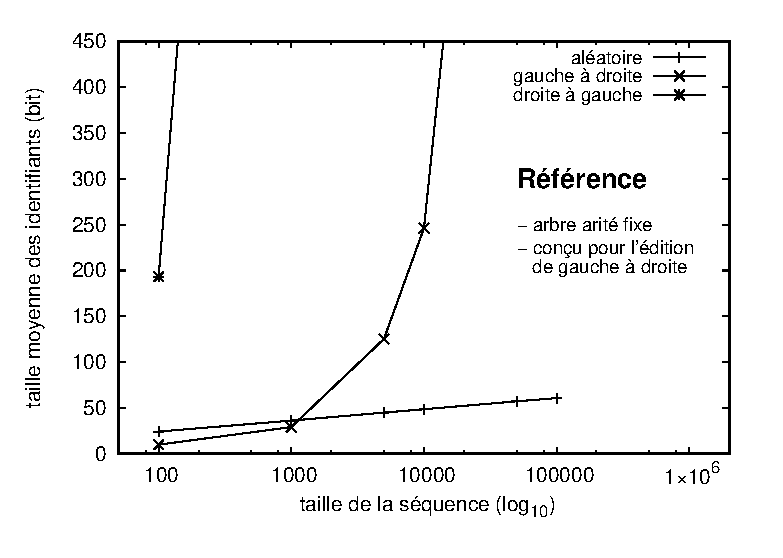
\includegraphics[width=1.25\textwidth]{img/replication/logoot.eps}
  \end{minipage}
  \hspace{1.5cm}
  \begin{minipage}{0.45\textwidth}
    \begin{tikzpicture}
      \node[visible on=<2-4>]
      {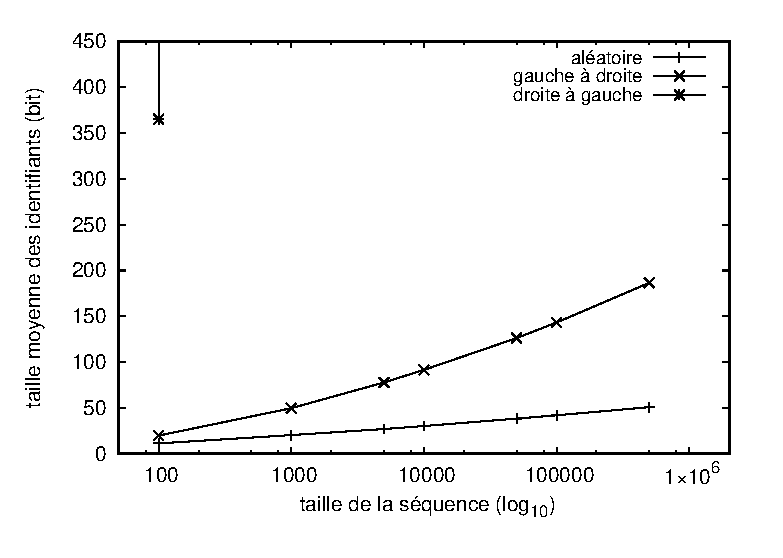
\includegraphics[width=1.25\textwidth]{img/replication/double.eps}};
    \end{tikzpicture}
  \end{minipage}
  
  \hspace{-1cm}
  \begin{minipage}{0.45\textwidth}
    \begin{tikzpicture}
      \node[visible on=<3-4>]
      {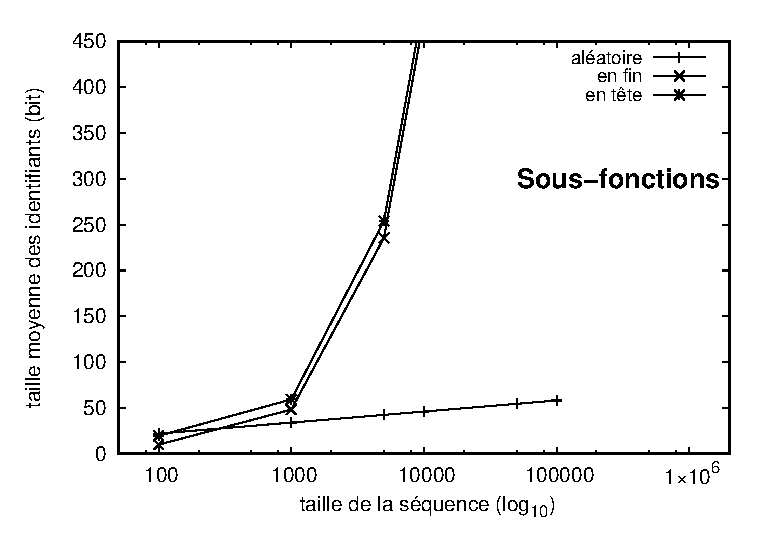
\includegraphics[width=1.25\textwidth]{img/replication/robin.eps}};
    \end{tikzpicture}
  \end{minipage}
  \hspace{1.5cm}
  \begin{minipage}{0.45\textwidth}
    \begin{tikzpicture}
      \node[visible on=<4-4>]
      {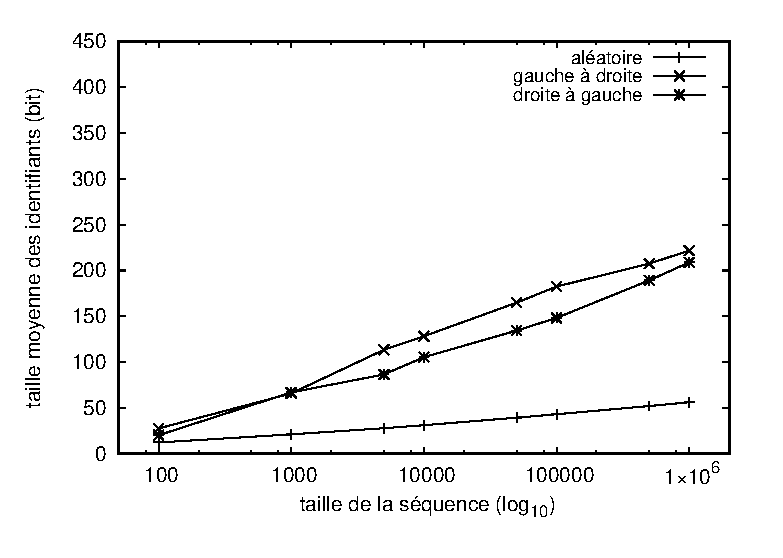
\includegraphics[width=1.25\textwidth]{img/replication/lseq.eps}};
    \end{tikzpicture}
  \end{minipage}

\end{frame}


\begin{frame}{Structure de séquences}{Identifiants sur traces réelles}

  \hspace{-1cm}
  \begin{minipage}{0.45\textwidth}
    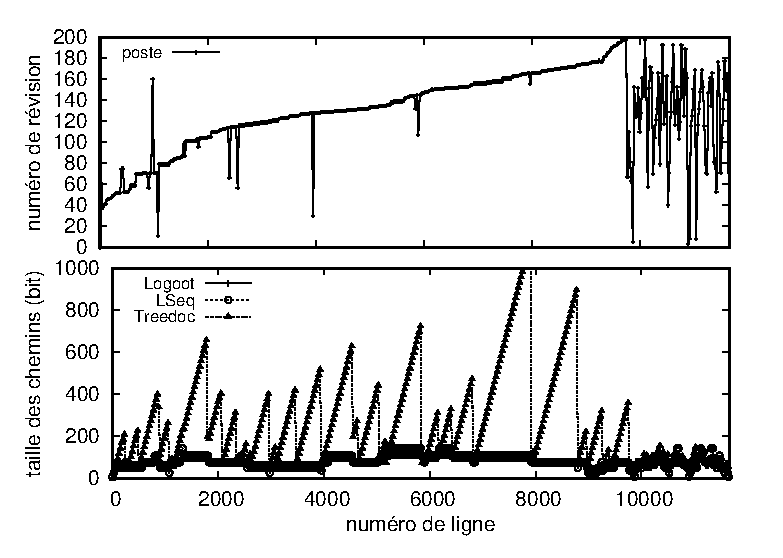
\includegraphics[width=1.29\textwidth]{img/replication/poste.eps}
  \end{minipage}
  \hspace{1.2cm}
  \begin{minipage}{0.45\textwidth}
    \begin{tikzpicture}
      \node[visible on=<2>]
      {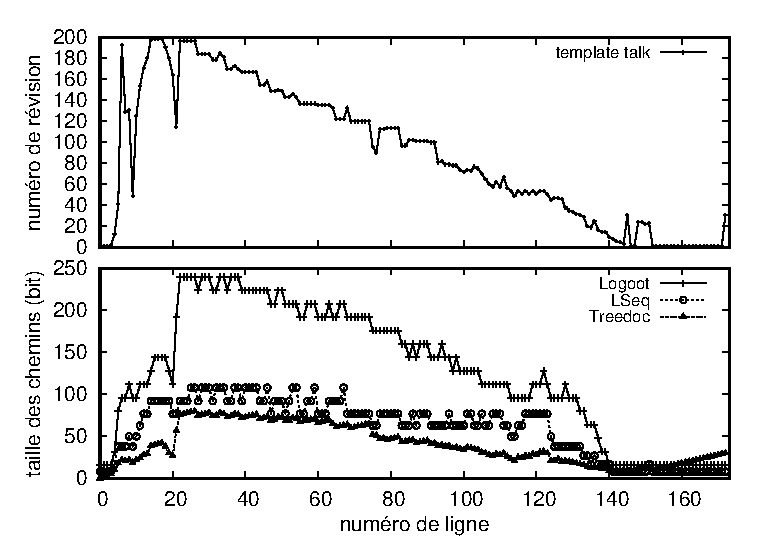
\includegraphics[width=1.29\textwidth]{img/replication/templatetalk.eps}};
    \end{tikzpicture}
  \end{minipage}

  \begin{minipage}{0.4\textwidth}
    Document édité en fin
  \end{minipage}
  \hspace{1.6cm}
  \begin{minipage}{0.4\textwidth}
    \begin{tikzpicture}
      \node[visible on=<2>]
      {Document édité au début};
    \end{tikzpicture}
  \end{minipage}


\end{frame}


\begin{frame}{Structure de séquences}{Évolution des performances}

  \begin{center}
    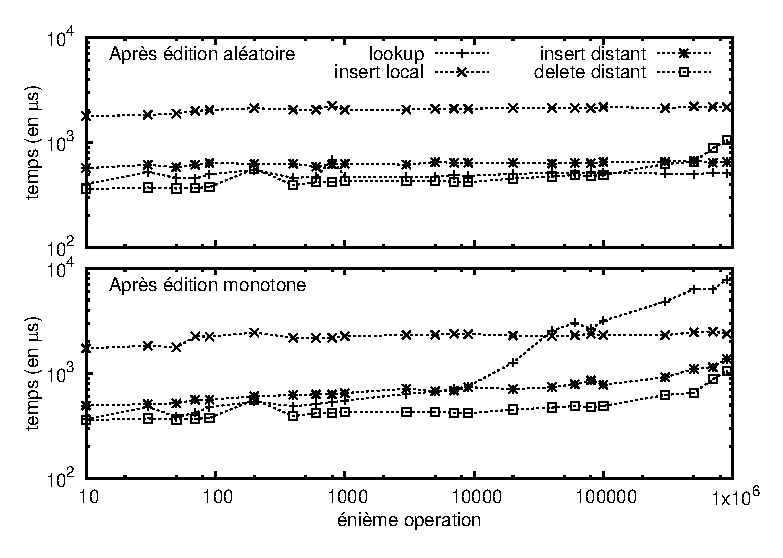
\includegraphics[width=\textwidth]{img/replication/time.eps}
  \end{center}

\end{frame}

\begin{frame}{Structure de séquences}{Effets de la concurrence}
  \vspace{-0.5cm}
  \begin{center}
    \includegraphics[angle=-90, width=\textwidth]{img/replication/latency.eps}
  \end{center}
\end{frame}

\begin{frame}{Structure de séquences}{Conclusion}

  \begin{itemize}
  \item \LSEQ est une fonction d'allocation d'identifiants pour les séquences
    réparties;
  \item Les identifiants générés ont une complexité sous-linéaire dans le contexte
    de l'édition collaborative
  \item [$\rightarrow$] ce qui répond partiellement au problème scientifique.
  \item [$\rightarrow$] Évite l'utilisation d'un méchanisme périodique de
    relocalisation dans l'édition collaborative.
  \end{itemize}


  \vspace{1cm}
  
  \large
  \begin{itemize}
  \item [$\Rightarrow$] Nécessite un moyen de communiquer les identifiants à tous
    les éditeurs.
  \end{itemize}

\end{frame}



%%% Local Variables:
%%% mode: latex
%%% TeX-master: "../slides"
%%% End:
